% Options for packages loaded elsewhere
\PassOptionsToPackage{unicode}{hyperref}
\PassOptionsToPackage{hyphens}{url}
%
\documentclass[
]{book}
\usepackage{lmodern}
\usepackage{amsmath}
\usepackage{ifxetex,ifluatex}
\ifnum 0\ifxetex 1\fi\ifluatex 1\fi=0 % if pdftex
  \usepackage[T1]{fontenc}
  \usepackage[utf8]{inputenc}
  \usepackage{textcomp} % provide euro and other symbols
  \usepackage{amssymb}
\else % if luatex or xetex
  \usepackage{unicode-math}
  \defaultfontfeatures{Scale=MatchLowercase}
  \defaultfontfeatures[\rmfamily]{Ligatures=TeX,Scale=1}
\fi
% Use upquote if available, for straight quotes in verbatim environments
\IfFileExists{upquote.sty}{\usepackage{upquote}}{}
\IfFileExists{microtype.sty}{% use microtype if available
  \usepackage[]{microtype}
  \UseMicrotypeSet[protrusion]{basicmath} % disable protrusion for tt fonts
}{}
\makeatletter
\@ifundefined{KOMAClassName}{% if non-KOMA class
  \IfFileExists{parskip.sty}{%
    \usepackage{parskip}
  }{% else
    \setlength{\parindent}{0pt}
    \setlength{\parskip}{6pt plus 2pt minus 1pt}}
}{% if KOMA class
  \KOMAoptions{parskip=half}}
\makeatother
\usepackage{xcolor}
\IfFileExists{xurl.sty}{\usepackage{xurl}}{} % add URL line breaks if available
\IfFileExists{bookmark.sty}{\usepackage{bookmark}}{\usepackage{hyperref}}
\hypersetup{
  pdftitle={My notes of ggplot2},
  pdfauthor={Matt Nickodemus},
  hidelinks,
  pdfcreator={LaTeX via pandoc}}
\urlstyle{same} % disable monospaced font for URLs
\usepackage{color}
\usepackage{fancyvrb}
\newcommand{\VerbBar}{|}
\newcommand{\VERB}{\Verb[commandchars=\\\{\}]}
\DefineVerbatimEnvironment{Highlighting}{Verbatim}{commandchars=\\\{\}}
% Add ',fontsize=\small' for more characters per line
\usepackage{framed}
\definecolor{shadecolor}{RGB}{248,248,248}
\newenvironment{Shaded}{\begin{snugshade}}{\end{snugshade}}
\newcommand{\AlertTok}[1]{\textcolor[rgb]{0.94,0.16,0.16}{#1}}
\newcommand{\AnnotationTok}[1]{\textcolor[rgb]{0.56,0.35,0.01}{\textbf{\textit{#1}}}}
\newcommand{\AttributeTok}[1]{\textcolor[rgb]{0.77,0.63,0.00}{#1}}
\newcommand{\BaseNTok}[1]{\textcolor[rgb]{0.00,0.00,0.81}{#1}}
\newcommand{\BuiltInTok}[1]{#1}
\newcommand{\CharTok}[1]{\textcolor[rgb]{0.31,0.60,0.02}{#1}}
\newcommand{\CommentTok}[1]{\textcolor[rgb]{0.56,0.35,0.01}{\textit{#1}}}
\newcommand{\CommentVarTok}[1]{\textcolor[rgb]{0.56,0.35,0.01}{\textbf{\textit{#1}}}}
\newcommand{\ConstantTok}[1]{\textcolor[rgb]{0.00,0.00,0.00}{#1}}
\newcommand{\ControlFlowTok}[1]{\textcolor[rgb]{0.13,0.29,0.53}{\textbf{#1}}}
\newcommand{\DataTypeTok}[1]{\textcolor[rgb]{0.13,0.29,0.53}{#1}}
\newcommand{\DecValTok}[1]{\textcolor[rgb]{0.00,0.00,0.81}{#1}}
\newcommand{\DocumentationTok}[1]{\textcolor[rgb]{0.56,0.35,0.01}{\textbf{\textit{#1}}}}
\newcommand{\ErrorTok}[1]{\textcolor[rgb]{0.64,0.00,0.00}{\textbf{#1}}}
\newcommand{\ExtensionTok}[1]{#1}
\newcommand{\FloatTok}[1]{\textcolor[rgb]{0.00,0.00,0.81}{#1}}
\newcommand{\FunctionTok}[1]{\textcolor[rgb]{0.00,0.00,0.00}{#1}}
\newcommand{\ImportTok}[1]{#1}
\newcommand{\InformationTok}[1]{\textcolor[rgb]{0.56,0.35,0.01}{\textbf{\textit{#1}}}}
\newcommand{\KeywordTok}[1]{\textcolor[rgb]{0.13,0.29,0.53}{\textbf{#1}}}
\newcommand{\NormalTok}[1]{#1}
\newcommand{\OperatorTok}[1]{\textcolor[rgb]{0.81,0.36,0.00}{\textbf{#1}}}
\newcommand{\OtherTok}[1]{\textcolor[rgb]{0.56,0.35,0.01}{#1}}
\newcommand{\PreprocessorTok}[1]{\textcolor[rgb]{0.56,0.35,0.01}{\textit{#1}}}
\newcommand{\RegionMarkerTok}[1]{#1}
\newcommand{\SpecialCharTok}[1]{\textcolor[rgb]{0.00,0.00,0.00}{#1}}
\newcommand{\SpecialStringTok}[1]{\textcolor[rgb]{0.31,0.60,0.02}{#1}}
\newcommand{\StringTok}[1]{\textcolor[rgb]{0.31,0.60,0.02}{#1}}
\newcommand{\VariableTok}[1]{\textcolor[rgb]{0.00,0.00,0.00}{#1}}
\newcommand{\VerbatimStringTok}[1]{\textcolor[rgb]{0.31,0.60,0.02}{#1}}
\newcommand{\WarningTok}[1]{\textcolor[rgb]{0.56,0.35,0.01}{\textbf{\textit{#1}}}}
\usepackage{longtable,booktabs}
\usepackage{calc} % for calculating minipage widths
% Correct order of tables after \paragraph or \subparagraph
\usepackage{etoolbox}
\makeatletter
\patchcmd\longtable{\par}{\if@noskipsec\mbox{}\fi\par}{}{}
\makeatother
% Allow footnotes in longtable head/foot
\IfFileExists{footnotehyper.sty}{\usepackage{footnotehyper}}{\usepackage{footnote}}
\makesavenoteenv{longtable}
\usepackage{graphicx}
\makeatletter
\def\maxwidth{\ifdim\Gin@nat@width>\linewidth\linewidth\else\Gin@nat@width\fi}
\def\maxheight{\ifdim\Gin@nat@height>\textheight\textheight\else\Gin@nat@height\fi}
\makeatother
% Scale images if necessary, so that they will not overflow the page
% margins by default, and it is still possible to overwrite the defaults
% using explicit options in \includegraphics[width, height, ...]{}
\setkeys{Gin}{width=\maxwidth,height=\maxheight,keepaspectratio}
% Set default figure placement to htbp
\makeatletter
\def\fps@figure{htbp}
\makeatother
\setlength{\emergencystretch}{3em} % prevent overfull lines
\providecommand{\tightlist}{%
  \setlength{\itemsep}{0pt}\setlength{\parskip}{0pt}}
\setcounter{secnumdepth}{5}
\usepackage{booktabs}
\usepackage{amsmath}
\usepackage{booktabs}
\usepackage{caption}
\usepackage{longtable}
\ifluatex
  \usepackage{selnolig}  % disable illegal ligatures
\fi
\usepackage[]{natbib}
\bibliographystyle{plainnat}

\title{My notes of ggplot2}
\author{Matt Nickodemus}
\date{2021-01-24}

\begin{document}
\maketitle

{
\setcounter{tocdepth}{1}
\tableofcontents
}
\hypertarget{disclaimer}{%
\chapter{Disclaimer}\label{disclaimer}}

These are my notes on ggplot. The thoughts, code, drawings, and notes are copied from several other sources, so \textbf{nothing here should be attributed to me}. This is just my notebook where I collect things I like as I learn.

\hypertarget{the-basics-of-ggplot2}{%
\chapter{The basics of ggplot2}\label{the-basics-of-ggplot2}}

Every layer in a ggplot has five components

\begin{itemize}
\tightlist
\item
  data
\item
  aesthetics
\item
  geom
\item
  stat
\item
  position
\end{itemize}

In addition to these five components we need to understand scales, guides, and themes. We will do this with a set of examples. Our first example is straight forward line plot showing the number of credits taken in each college from 2011 to 2020. As we walk though this, we will look at three components

\begin{itemize}
\tightlist
\item
  data
\item
  aesthetics
\item
  geom
\end{itemize}

and

\begin{itemize}
\tightlist
\item
  scales
\item
  guides
\item
  themes
\end{itemize}

\hypertarget{data}{%
\section{Data}\label{data}}

We will create a data set consisting of college credit counts for 2011-2020.

\begin{Shaded}
\begin{Highlighting}[]
\FunctionTok{library}\NormalTok{(tidyverse)}
\FunctionTok{library}\NormalTok{(purrr)}

\NormalTok{make\_credits }\OtherTok{\textless{}{-}} \ControlFlowTok{function}\NormalTok{(college) \{}
\NormalTok{  slope }\OtherTok{\textless{}{-}} \FunctionTok{rnorm}\NormalTok{(}\DecValTok{1}\NormalTok{, }\DecValTok{500}\NormalTok{, }\DecValTok{500}\NormalTok{)}
\NormalTok{  intercept }\OtherTok{\textless{}{-}} \FunctionTok{rnorm}\NormalTok{(}\DecValTok{1}\NormalTok{, }\DecValTok{20000}\NormalTok{, }\DecValTok{2000}\NormalTok{) }\SpecialCharTok{\%\textgreater{}\%} \FunctionTok{floor}\NormalTok{()}
\NormalTok{  x }\OtherTok{\textless{}{-}} \DecValTok{1}\SpecialCharTok{:}\DecValTok{10}
\NormalTok{  college }\OtherTok{\textless{}{-}} \FunctionTok{rep}\NormalTok{(college, }\DecValTok{10}\NormalTok{)}
\NormalTok{  noise }\OtherTok{\textless{}{-}} \FunctionTok{rnorm}\NormalTok{(}\DecValTok{10}\NormalTok{, }\DecValTok{1000}\NormalTok{, }\DecValTok{1000}\NormalTok{)}
  
\NormalTok{  credits }\OtherTok{\textless{}{-}}\NormalTok{ intercept }\SpecialCharTok{+}\NormalTok{ slope}\SpecialCharTok{*}\NormalTok{x }\SpecialCharTok{+}\NormalTok{ noise}
  
\NormalTok{  output\_df }\OtherTok{\textless{}{-}} \FunctionTok{tibble}\NormalTok{(}\AttributeTok{college =}\NormalTok{ college, }\AttributeTok{year =} \DecValTok{2010} \SpecialCharTok{+}\NormalTok{ x, }\AttributeTok{credits =}\NormalTok{ credits ) }\SpecialCharTok{\%\textgreater{}\%} 
    \FunctionTok{mutate}\NormalTok{(}\AttributeTok{credits =} \FunctionTok{as.integer}\NormalTok{(credits))}
  
  \FunctionTok{return}\NormalTok{(output\_df)}
\NormalTok{\}}


\NormalTok{colleges }\OtherTok{\textless{}{-}} \FunctionTok{c}\NormalTok{(}\StringTok{\textquotesingle{}Fine Art\textquotesingle{}}\NormalTok{, }\StringTok{\textquotesingle{}Business\textquotesingle{}}\NormalTok{, }\StringTok{\textquotesingle{}Physical Science\textquotesingle{}}\NormalTok{, }\StringTok{\textquotesingle{}Social Science\textquotesingle{}}\NormalTok{, }
              \StringTok{\textquotesingle{}Health Science\textquotesingle{}}\NormalTok{, }\StringTok{\textquotesingle{}Humanities\textquotesingle{}}\NormalTok{, }\StringTok{\textquotesingle{}Life Science\textquotesingle{}}\NormalTok{, }\StringTok{\textquotesingle{}Earl\textquotesingle{}}\NormalTok{)}

\NormalTok{credits\_by\_college }\OtherTok{\textless{}{-}} \FunctionTok{map\_dfr}\NormalTok{(colleges, make\_credits)}
\end{Highlighting}
\end{Shaded}

This data output is in tidy format. In tidy data

\begin{itemize}
\tightlist
\item
  Each variable forms a column.
\item
  Each observation forms a row.
\item
  Each type of observational unit forms a table.
\end{itemize}

For our data set, the observations are the number of credits offered by a specific
college in a given term. The variables are year and credits. Your data should always be tidy when using ggplot.

\begin{Shaded}
\begin{Highlighting}[]
\FunctionTok{library}\NormalTok{(gt)}
\FunctionTok{head}\NormalTok{(credits\_by\_college) }\SpecialCharTok{\%\textgreater{}\%} \FunctionTok{gt}\NormalTok{()}
\end{Highlighting}
\end{Shaded}

\captionsetup[table]{labelformat=empty,skip=1pt}
\begin{longtable}{lrc}
\toprule
college & year & credits \\ 
\midrule
Fine Art & 2011 & 24746 \\ 
Fine Art & 2012 & 25620 \\ 
Fine Art & 2013 & 25761 \\ 
Fine Art & 2014 & 26837 \\ 
Fine Art & 2015 & 24846 \\ 
Fine Art & 2016 & 29265 \\ 
\bottomrule
\end{longtable}

In our plot the data layer is created with the following code. Note that there is nothing on plot. There are no axes, no graphs, no colors, no legend. Just a blank canvas. The reason for this is that in ggplot, the plot is created when we map the variables in the data to visual elements in the plot. This is done with the aes() function.

\begin{Shaded}
\begin{Highlighting}[]
\FunctionTok{ggplot}\NormalTok{(credits\_by\_college)}
\end{Highlighting}
\end{Shaded}


\includegraphics{notes_ggplot_files/figure-latex/unnamed-chunk-3-1.pdf}

\hypertarget{aesthetics}{%
\section{aesthetics}\label{aesthetics}}

When we add the \texttt{aes()} call within the \texttt{ggplot} call, we produce a set of axes on our plot. This is because we have mapped the variable year to the x axis in our graph, and the variable credits to the y-axis in our graph. We do not see a plot yet because we have not yet told ggplot what type of geometric object we want to use to in our plot. We do that next.

\begin{Shaded}
\begin{Highlighting}[]
\FunctionTok{ggplot}\NormalTok{(credits\_by\_college, }\FunctionTok{aes}\NormalTok{(}\AttributeTok{x =}\NormalTok{ year, }\AttributeTok{y =}\NormalTok{ credits))}
\end{Highlighting}
\end{Shaded}

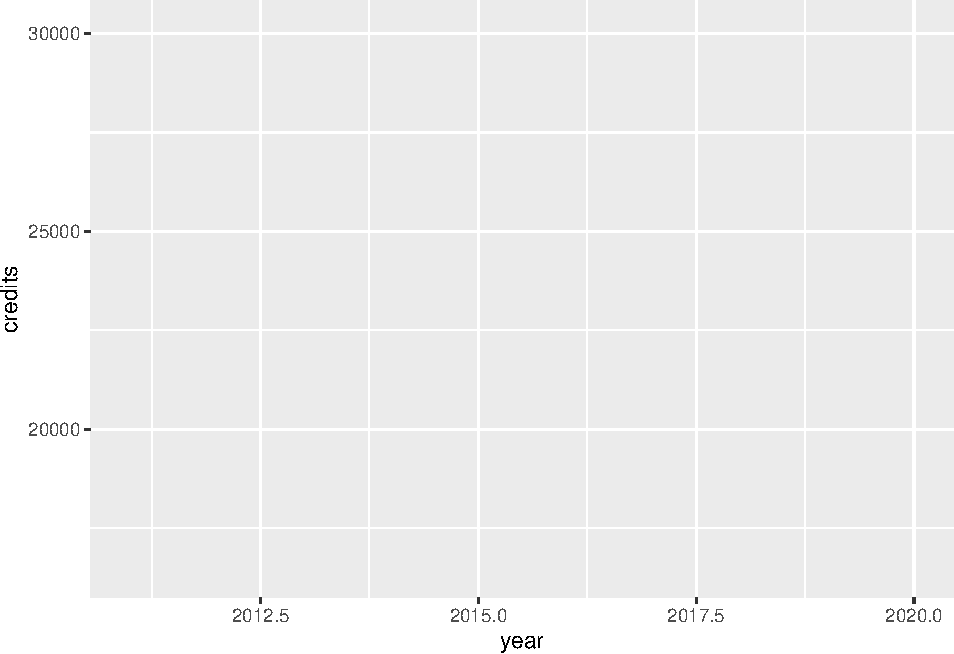
\includegraphics{notes_ggplot_files/figure-latex/unnamed-chunk-4-1.pdf}

\hypertarget{geom}{%
\section{geom}\label{geom}}

\hypertarget{wtf}{%
\subsection{WTF}\label{wtf}}

In our next plot we have chosen the line geom for our graph. This does not give us the result that we are looking for. We are trying to draw a line chart showing credits for each year, for each college. The mistake we have made is that we have not assigned the college variable to as visual aspect of our graph. We do so in the next graph.

\begin{Shaded}
\begin{Highlighting}[]
\FunctionTok{ggplot}\NormalTok{(credits\_by\_college, }\FunctionTok{aes}\NormalTok{(}\AttributeTok{x =}\NormalTok{ year, }\AttributeTok{y =}\NormalTok{ credits)) }\SpecialCharTok{+} \FunctionTok{geom\_line}\NormalTok{()}
\end{Highlighting}
\end{Shaded}

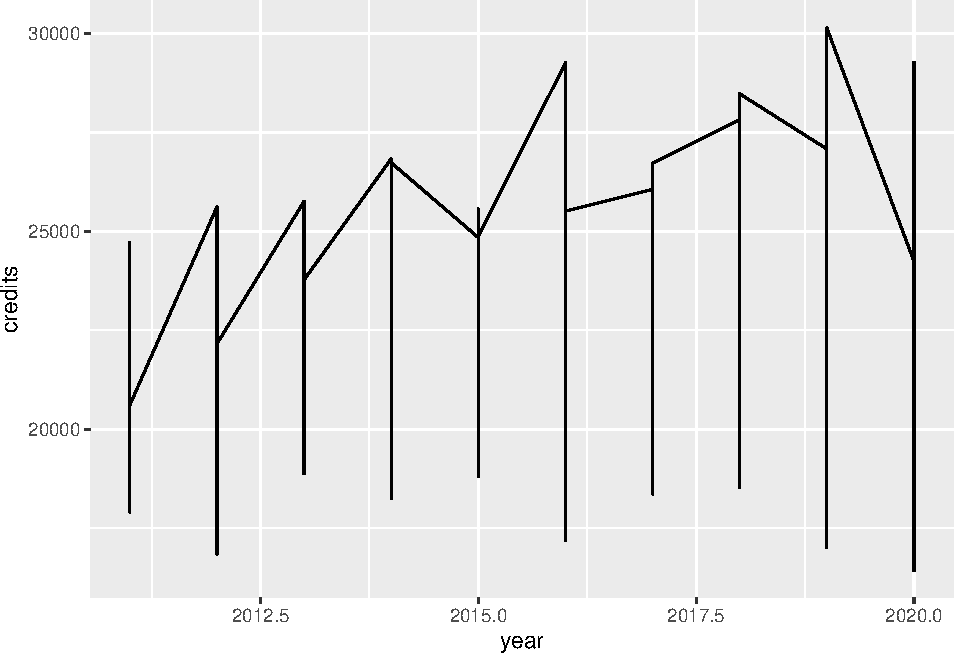
\includegraphics{notes_ggplot_files/figure-latex/unnamed-chunk-5-1.pdf}

\hypertarget{more-aesthetics}{%
\subsection{More aesthetics?}\label{more-aesthetics}}

This graph gives us something closer to what we are looking for, but it is still not quite there.

\begin{Shaded}
\begin{Highlighting}[]
\FunctionTok{ggplot}\NormalTok{(credits\_by\_college, }\FunctionTok{aes}\NormalTok{(}\AttributeTok{x =}\NormalTok{ year, }\AttributeTok{y =}\NormalTok{ credits, }\AttributeTok{group =}\NormalTok{ college)) }\SpecialCharTok{+} \FunctionTok{geom\_line}\NormalTok{()}
\end{Highlighting}
\end{Shaded}

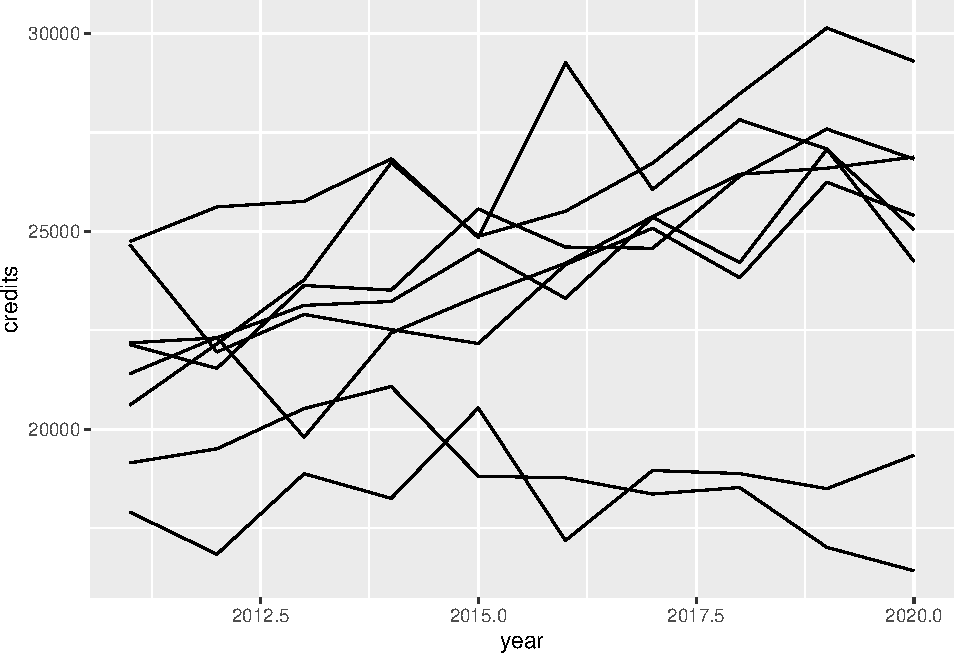
\includegraphics{notes_ggplot_files/figure-latex/unnamed-chunk-6-1.pdf}

The problem is that we would like the lines to be different colors, and we would like each color to be associated with a color. So we have to map the variable college to another aesthetic, color.

\begin{Shaded}
\begin{Highlighting}[]
\FunctionTok{ggplot}\NormalTok{(credits\_by\_college, }\FunctionTok{aes}\NormalTok{(}\AttributeTok{x =}\NormalTok{ year, }\AttributeTok{y =}\NormalTok{ credits, }\AttributeTok{group =}\NormalTok{ college, }\AttributeTok{color =}\NormalTok{ college)) }\SpecialCharTok{+} 
  \FunctionTok{geom\_line}\NormalTok{() }\SpecialCharTok{+} \FunctionTok{geom\_point}\NormalTok{(}\AttributeTok{size =}\NormalTok{ .}\DecValTok{5}\NormalTok{, }\AttributeTok{alpha =}\NormalTok{ .}\DecValTok{8}\NormalTok{)}
\end{Highlighting}
\end{Shaded}

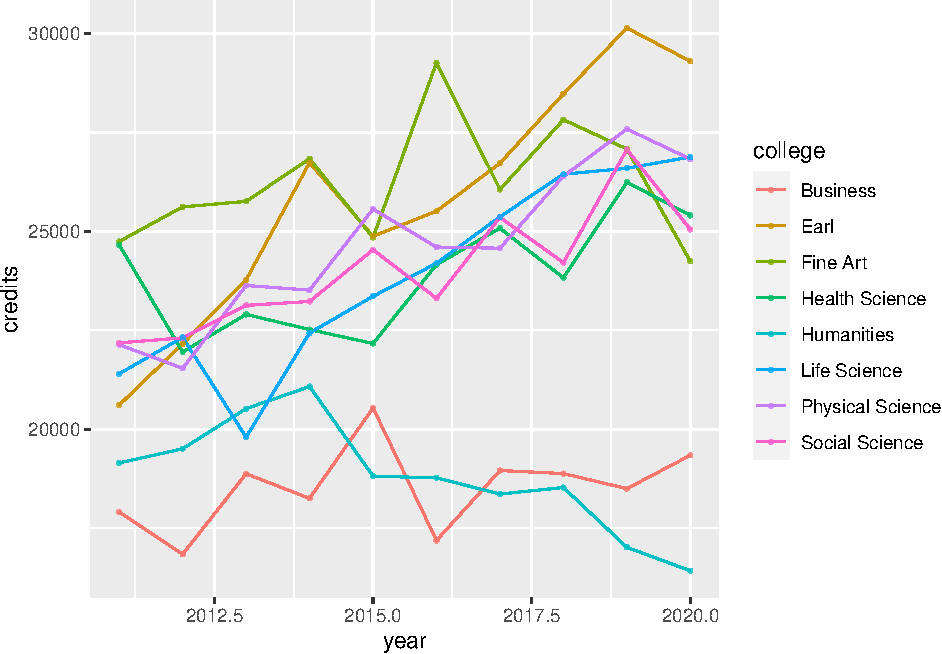
\includegraphics{notes_ggplot_files/figure-latex/unnamed-chunk-7-1.pdf}

\hypertarget{scale}{%
\section{Scale}\label{scale}}

\begin{Shaded}
\begin{Highlighting}[]
\FunctionTok{library}\NormalTok{(scales)}
\end{Highlighting}
\end{Shaded}

\begin{verbatim}
## 
## Attaching package: 'scales'
\end{verbatim}

\begin{verbatim}
## The following object is masked from 'package:purrr':
## 
##     discard
\end{verbatim}

\begin{verbatim}
## The following object is masked from 'package:readr':
## 
##     col_factor
\end{verbatim}

\begin{Shaded}
\begin{Highlighting}[]
\FunctionTok{ggplot}\NormalTok{(credits\_by\_college, }\FunctionTok{aes}\NormalTok{(}\AttributeTok{x =}\NormalTok{ year, }\AttributeTok{y =}\NormalTok{ credits, }\AttributeTok{group =}\NormalTok{ college, }\AttributeTok{color =}\NormalTok{ college)) }\SpecialCharTok{+} 
  \FunctionTok{geom\_line}\NormalTok{() }\SpecialCharTok{+} \FunctionTok{geom\_point}\NormalTok{(}\AttributeTok{size =}\NormalTok{ .}\DecValTok{5}\NormalTok{, }\AttributeTok{alpha =}\NormalTok{ .}\DecValTok{8}\NormalTok{) }\SpecialCharTok{+}
  \FunctionTok{scale\_x\_continuous}\NormalTok{(}\AttributeTok{breaks =} \FunctionTok{pretty\_breaks}\NormalTok{()) }\SpecialCharTok{+}
  \FunctionTok{scale\_y\_continuous}\NormalTok{(}\AttributeTok{labels =}\NormalTok{ comma)}
\end{Highlighting}
\end{Shaded}

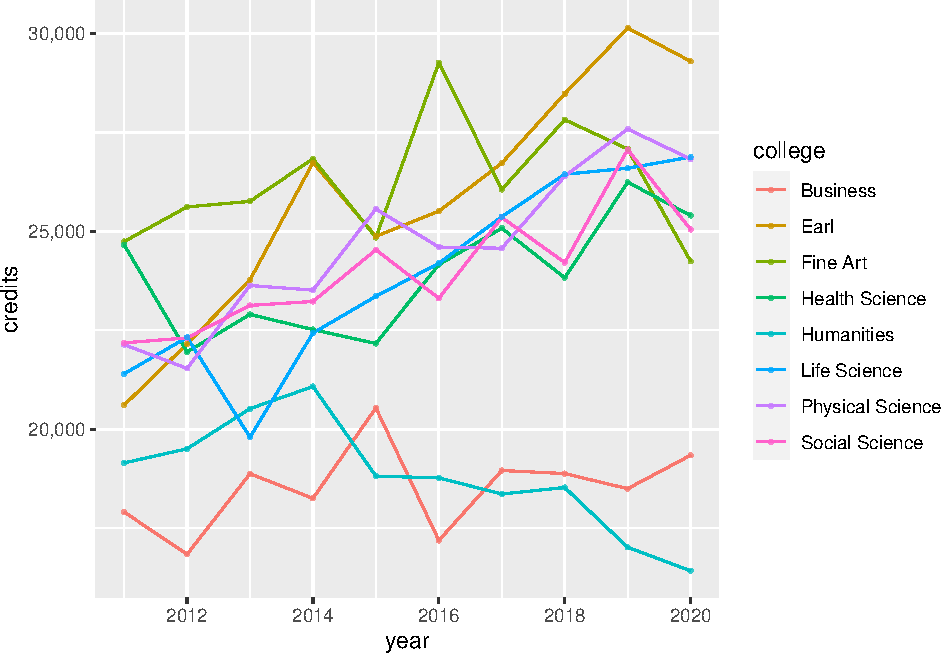
\includegraphics{notes_ggplot_files/figure-latex/unnamed-chunk-8-1.pdf}

\hypertarget{guide}{%
\section{Guide}\label{guide}}

\begin{Shaded}
\begin{Highlighting}[]
\FunctionTok{ggplot}\NormalTok{(credits\_by\_college, }\FunctionTok{aes}\NormalTok{(}\AttributeTok{x =}\NormalTok{ year, }\AttributeTok{y =}\NormalTok{ credits, }\AttributeTok{group =}\NormalTok{ college, }\AttributeTok{color =}\NormalTok{ college)) }\SpecialCharTok{+} 
  \FunctionTok{geom\_line}\NormalTok{() }\SpecialCharTok{+} \FunctionTok{geom\_point}\NormalTok{(}\AttributeTok{size =}\NormalTok{ .}\DecValTok{5}\NormalTok{, }\AttributeTok{alpha =}\NormalTok{ .}\DecValTok{8}\NormalTok{) }\SpecialCharTok{+}
  \FunctionTok{scale\_x\_continuous}\NormalTok{(}\AttributeTok{breaks =} \FunctionTok{pretty\_breaks}\NormalTok{()) }\SpecialCharTok{+}
  \FunctionTok{scale\_y\_continuous}\NormalTok{(}\AttributeTok{labels =}\NormalTok{ comma) }\SpecialCharTok{+}
  \FunctionTok{guides}\NormalTok{(}\AttributeTok{color =} \FunctionTok{guide\_legend}\NormalTok{(}\AttributeTok{title =} \StringTok{"College"}\NormalTok{))}
\end{Highlighting}
\end{Shaded}

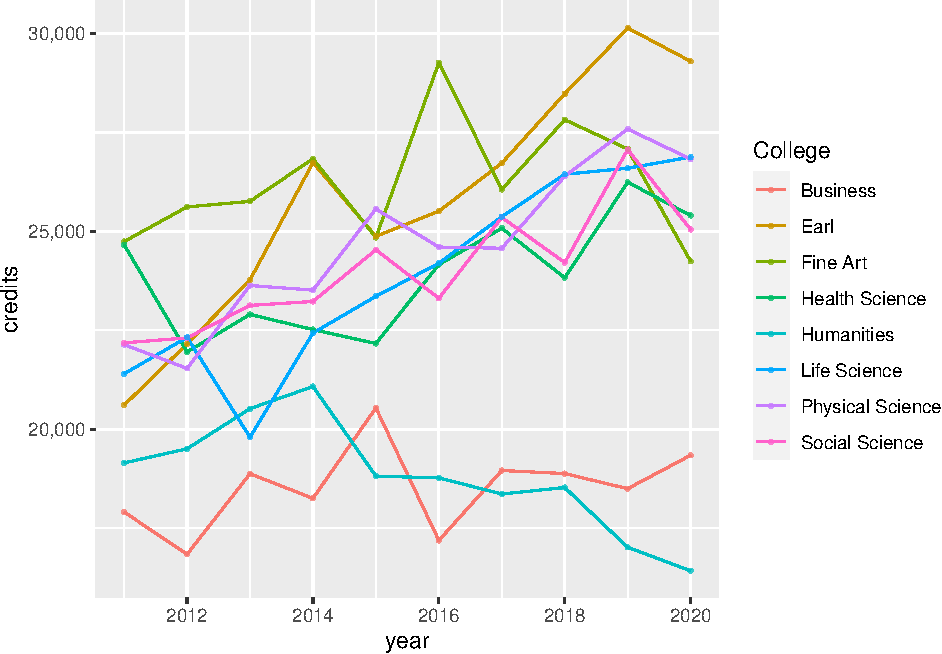
\includegraphics{notes_ggplot_files/figure-latex/unnamed-chunk-9-1.pdf}

\hypertarget{labels}{%
\section{Labels}\label{labels}}

\begin{Shaded}
\begin{Highlighting}[]
\FunctionTok{ggplot}\NormalTok{(credits\_by\_college, }\FunctionTok{aes}\NormalTok{(}\AttributeTok{x =}\NormalTok{ year, }\AttributeTok{y =}\NormalTok{ credits, }\AttributeTok{group =}\NormalTok{ college, }\AttributeTok{color =}\NormalTok{ college)) }\SpecialCharTok{+} 
  \FunctionTok{geom\_line}\NormalTok{() }\SpecialCharTok{+} \FunctionTok{geom\_point}\NormalTok{(}\AttributeTok{size =}\NormalTok{ .}\DecValTok{5}\NormalTok{, }\AttributeTok{alpha =}\NormalTok{ .}\DecValTok{8}\NormalTok{) }\SpecialCharTok{+}
  \FunctionTok{scale\_x\_continuous}\NormalTok{(}\AttributeTok{breaks =} \FunctionTok{pretty\_breaks}\NormalTok{()) }\SpecialCharTok{+}
  \FunctionTok{scale\_y\_continuous}\NormalTok{(}\AttributeTok{labels =}\NormalTok{ comma) }\SpecialCharTok{+}
  \FunctionTok{guides}\NormalTok{(}\AttributeTok{color =} \FunctionTok{guide\_legend}\NormalTok{(}\AttributeTok{title =} \StringTok{"College"}\NormalTok{)) }\SpecialCharTok{+}
  \FunctionTok{labs}\NormalTok{(}\AttributeTok{title =} \StringTok{"Credits by college"}\NormalTok{,}
       \AttributeTok{subtitle =} \StringTok{"Credits taken within each college 2011{-}2020"}\NormalTok{,}
       \AttributeTok{caption =} \StringTok{"Data supplied by OIE"}\NormalTok{) }\SpecialCharTok{+}
  \FunctionTok{xlab}\NormalTok{(}\StringTok{"Year"}\NormalTok{) }\SpecialCharTok{+}
  \FunctionTok{ylab}\NormalTok{(}\StringTok{\textquotesingle{}Credits\textquotesingle{}}\NormalTok{)}
\end{Highlighting}
\end{Shaded}

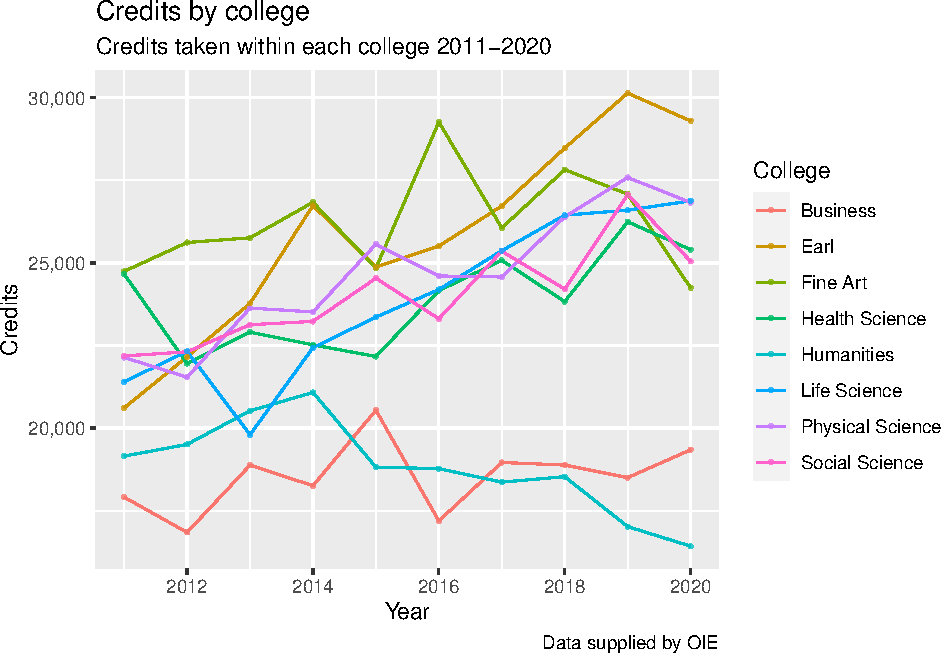
\includegraphics{notes_ggplot_files/figure-latex/unnamed-chunk-10-1.pdf}

\hypertarget{theme}{%
\section{Theme}\label{theme}}

\begin{Shaded}
\begin{Highlighting}[]
\FunctionTok{ggplot}\NormalTok{(credits\_by\_college, }\FunctionTok{aes}\NormalTok{(}\AttributeTok{x =}\NormalTok{ year, }\AttributeTok{y =}\NormalTok{ credits, }\AttributeTok{group =}\NormalTok{ college, }\AttributeTok{color =}\NormalTok{ college)) }\SpecialCharTok{+} 
  \FunctionTok{geom\_line}\NormalTok{() }\SpecialCharTok{+} \FunctionTok{geom\_point}\NormalTok{(}\AttributeTok{size =}\NormalTok{ .}\DecValTok{5}\NormalTok{, }\AttributeTok{alpha =}\NormalTok{ .}\DecValTok{8}\NormalTok{) }\SpecialCharTok{+}
  \FunctionTok{scale\_x\_continuous}\NormalTok{(}\AttributeTok{breaks =} \FunctionTok{pretty\_breaks}\NormalTok{()) }\SpecialCharTok{+}
  \FunctionTok{scale\_y\_continuous}\NormalTok{(}\AttributeTok{labels =}\NormalTok{ comma) }\SpecialCharTok{+}
  \FunctionTok{guides}\NormalTok{(}\AttributeTok{color =} \FunctionTok{guide\_legend}\NormalTok{(}\AttributeTok{title =} \StringTok{"College"}\NormalTok{)) }\SpecialCharTok{+}
  \FunctionTok{labs}\NormalTok{(}\AttributeTok{title =} \StringTok{"Credits by college"}\NormalTok{,}
       \AttributeTok{subtitle =} \StringTok{"Credits taken within each college 2011{-}2020"}\NormalTok{,}
       \AttributeTok{caption =} \StringTok{"Data supplied by OIE"}\NormalTok{,}
       \AttributeTok{x =} \StringTok{\textquotesingle{}Year\textquotesingle{}}\NormalTok{,}
       \AttributeTok{y =} \StringTok{\textquotesingle{}Credits\textquotesingle{}}\NormalTok{) }\SpecialCharTok{+}
  \FunctionTok{theme\_minimal}\NormalTok{() }\SpecialCharTok{+}
  \FunctionTok{theme}\NormalTok{(}
    \AttributeTok{panel.grid.major.x =} \FunctionTok{element\_blank}\NormalTok{(),}
    \AttributeTok{panel.grid.minor.x =} \FunctionTok{element\_blank}\NormalTok{(),}
    \AttributeTok{panel.grid.minor.y =} \FunctionTok{element\_blank}\NormalTok{(),}
    \AttributeTok{plot.subtitle =} \FunctionTok{element\_text}\NormalTok{(}\AttributeTok{color =} \StringTok{"\#a6a6a6"}\NormalTok{, }\AttributeTok{size =} \DecValTok{10}\NormalTok{),}
    \AttributeTok{plot.caption =} \FunctionTok{element\_text}\NormalTok{(}\AttributeTok{color =} \StringTok{\textquotesingle{}\#a6a6a6\textquotesingle{}}\NormalTok{, }\AttributeTok{size =} \DecValTok{8}\NormalTok{, }\AttributeTok{face =} \StringTok{\textquotesingle{}italic\textquotesingle{}}\NormalTok{)}
\NormalTok{  )}
\end{Highlighting}
\end{Shaded}

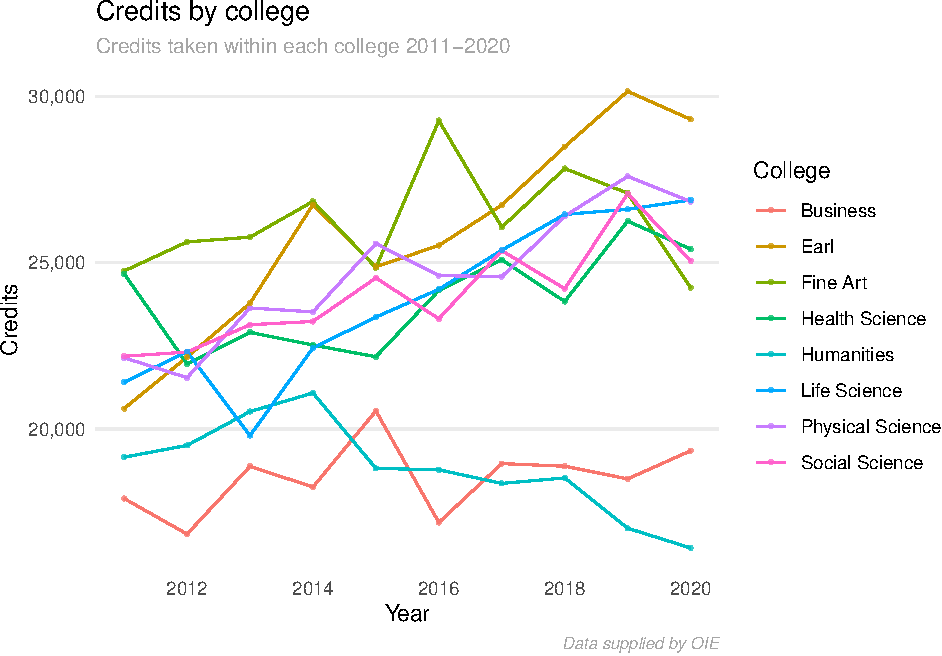
\includegraphics{notes_ggplot_files/figure-latex/unnamed-chunk-11-1.pdf}

\end{document}
